% This file was created with tikzplotlib v0.10.1.
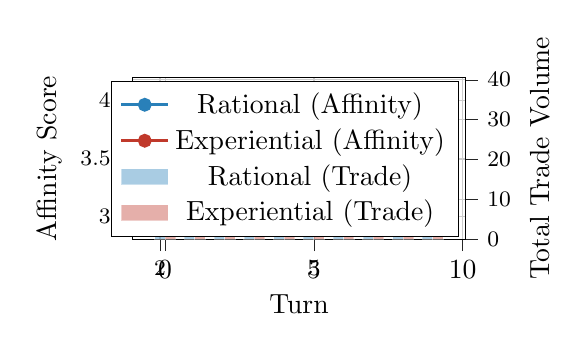
\begin{tikzpicture}

\definecolor{darkslategrey38}{RGB}{38,38,38}
\definecolor{firebrick1925743}{RGB}{192,57,43}
\definecolor{lightgrey204}{RGB}{204,204,204}
\definecolor{steelblue41128185}{RGB}{41,128,185}

\begin{axis}[
   width=0.48\textwidth,
   height=0.3\textwidth,
   axis line style={black},
   tick align=outside,
   x grid style={lightgrey204},
   xlabel=Turn,
   xlabel style={font=\footnotesize, yshift=5pt},
   %xtick={0,1,2,3,4,5,6,7,8,9},
   xticklabels={1,2,3,4,5,6,7,8,9,10},
   xticklabel style={font=\footnotesize},
   ylabel=Affinity Score,
   ylabel style={font=\footnotesize, inner sep=0pt, yshift=-5pt},
   ymajorgrids,
   ymin=2.8, ymax=4.2,
   yticklabel style={font=\footnotesize},
   grid=major,
   grid style={lightgrey204},
   tick style={color=darkslategrey38},
   axis lines=box,
   x axis line style={black},
   y axis line style={black},
   tick pos=left,
   xtick pos=bottom,
   clip=true
]
\path [draw=steelblue41128185, fill=steelblue41128185, opacity=0.2]
(axis cs:0,3.6)
--(axis cs:0,3.25)
--(axis cs:1,3.4)
--(axis cs:2,3.48333333333333)
--(axis cs:3,3.66666666666667)
--(axis cs:4,3.56666666666667)
--(axis cs:5,3.4)
--(axis cs:6,3.36625)
--(axis cs:7,3.21666666666667)
--(axis cs:8,3.16666666666667)
--(axis cs:9,3.08333333333333)
--(axis cs:9,3.68333333333333)
--(axis cs:9,3.68333333333333)
--(axis cs:8,3.78333333333333)
--(axis cs:7,3.81666666666667)
--(axis cs:6,3.9)
--(axis cs:5,3.90041666666667)
--(axis cs:4,4.03333333333333)
--(axis cs:3,4.08333333333333)
--(axis cs:2,3.85)
--(axis cs:1,3.78333333333333)
--(axis cs:0,3.6)
--cycle;

\path [draw=firebrick1925743, fill=firebrick1925743, opacity=0.2]
(axis cs:0,3.56666666666667)
--(axis cs:0,3.19958333333333)
--(axis cs:1,3.11666666666667)
--(axis cs:2,3.05)
--(axis cs:3,3.1)
--(axis cs:4,3.2)
--(axis cs:5,3.33333333333333)
--(axis cs:6,3.3)
--(axis cs:7,3.29958333333333)
--(axis cs:8,3.15)
--(axis cs:9,3.15)
--(axis cs:9,3.75)
--(axis cs:9,3.75)
--(axis cs:8,3.68333333333333)
--(axis cs:7,3.88333333333333)
--(axis cs:6,3.91666666666667)
--(axis cs:5,3.86666666666667)
--(axis cs:4,3.75)
--(axis cs:3,3.58333333333333)
--(axis cs:2,3.5)
--(axis cs:1,3.53333333333333)
--(axis cs:0,3.56666666666667)
--cycle;

\addplot [line width=1pt, steelblue41128185, mark=*, mark size=3, mark options={solid,draw=white}]
table {%
0 3.43333333333333
1 3.6
2 3.66666666666667
3 3.88333333333333
4 3.8
5 3.66666666666667
6 3.63333333333333
7 3.5
8 3.46666666666667
9 3.38333333333333
};
\addplot [line width=1pt, firebrick1925743, mark=*, mark size=3, mark options={solid,draw=white}]
table {%
0 3.38333333333333
1 3.33333333333333
2 3.28333333333333
3 3.33333333333333
4 3.5
5 3.6
6 3.63333333333333
7 3.6
8 3.41666666666667
9 3.45
};
\end{axis}

\begin{axis}[
   width=0.48\textwidth,
   height=0.3\textwidth,
   axis y line=right,
   tick align=outside,
   x grid style={lightgrey204},
   % xtick={0,1,2,3,4,5,6,7,8,9},
   % xticklabels={1,2,3,4,5,6,7,8,9,10},
   ylabel=Total Trade Volume,
   ylabel style={font=\footnotesize, inner sep=0pt, yshift=-5pt},
   ymajorgrids,
   ymin=0, ymax=40.5968743769439,
   yticklabel style={font=\footnotesize, anchor=west},
   grid=major,
   grid style={lightgrey204},
   tick style={color=darkslategrey38},
   axis lines=box,
   x axis line style={black},
   y axis line style={black},
   tick pos=right,
   xtick pos=bottom,
   clip=true
]
\draw[draw=white,fill=steelblue41128185,opacity=0.4] (axis cs:-0.35,0) rectangle (axis cs:0,10.9);

\addlegendimage{color=steelblue41128185, mark=*, mark size=2pt, line width=1pt}
\addlegendimage{color=firebrick1925743, mark=*, mark size=2pt, line width=1pt}
% \addlegendimage{ybar,ybar legend,draw=white,fill=steelblue41128185,opacity=0.4}
% \addlegendimage{ybar,ybar legend,draw=white,fill=firebrick1925743,opacity=0.4}
\addlegendimage{area legend, draw=white, fill=steelblue41128185, opacity=0.4}
\addlegendimage{area legend, draw=white, fill=firebrick1925743, opacity=0.4}
\addlegendentry{Rational (Affinity)}
\addlegendentry{Experiential (Affinity)}
\addlegendentry{Rational (Trade)}
\addlegendentry{Experiential (Trade)}
% \addlegendimage{ybar,ybar legend,draw=white,fill=steelblue41128185,opacity=0.4}
% \addlegendentry{Rational (Trade)}

\draw[draw=white,fill=steelblue41128185,opacity=0.4] (axis cs:0.65,0) rectangle (axis cs:1,12.5);
\draw[draw=white,fill=steelblue41128185,opacity=0.4] (axis cs:1.65,0) rectangle (axis cs:2,15.5);
\draw[draw=white,fill=steelblue41128185,opacity=0.4] (axis cs:2.65,0) rectangle (axis cs:3,21.8);
\draw[draw=white,fill=steelblue41128185,opacity=0.4] (axis cs:3.65,0) rectangle (axis cs:4,24.4444444444444);
\draw[draw=white,fill=steelblue41128185,opacity=0.4] (axis cs:4.65,0) rectangle (axis cs:5,27.4);
\draw[draw=white,fill=steelblue41128185,opacity=0.4] (axis cs:5.65,0) rectangle (axis cs:6,28.3333333333333);
\draw[draw=white,fill=steelblue41128185,opacity=0.4] (axis cs:6.65,0) rectangle (axis cs:7,27.6);
\draw[draw=white,fill=steelblue41128185,opacity=0.4] (axis cs:7.65,0) rectangle (axis cs:8,32.1111111111111);
\draw[draw=white,fill=steelblue41128185,opacity=0.4] (axis cs:8.65,0) rectangle (axis cs:9,28.3333333333333);
\draw[draw=white,fill=firebrick1925743,opacity=0.4] (axis cs:2.77555756156289e-17,0) rectangle (axis cs:0.35,11.5);
% \addlegendimage{ybar,ybar legend,draw=white,fill=firebrick1925743,opacity=0.4}
% \addlegendentry{Experiential (Trade)}

\draw[draw=white,fill=firebrick1925743,opacity=0.4] (axis cs:1,0) rectangle (axis cs:1.35,10.2);
\draw[draw=white,fill=firebrick1925743,opacity=0.4] (axis cs:2,0) rectangle (axis cs:2.35,11.9);
\draw[draw=white,fill=firebrick1925743,opacity=0.4] (axis cs:3,0) rectangle (axis cs:3.35,14.7);
\draw[draw=white,fill=firebrick1925743,opacity=0.4] (axis cs:4,0) rectangle (axis cs:4.35,17.9);
\draw[draw=white,fill=firebrick1925743,opacity=0.4] (axis cs:5,0) rectangle (axis cs:5.35,22.4);
\draw[draw=white,fill=firebrick1925743,opacity=0.4] (axis cs:6,0) rectangle (axis cs:6.35,29.5555555555556);
\draw[draw=white,fill=firebrick1925743,opacity=0.4] (axis cs:7,0) rectangle (axis cs:7.35,26.6666666666667);
\draw[draw=white,fill=firebrick1925743,opacity=0.4] (axis cs:8,0) rectangle (axis cs:8.35,25.6666666666667);
\draw[draw=white,fill=firebrick1925743,opacity=0.4] (axis cs:9,0) rectangle (axis cs:9.35,31.2);
\path [draw=steelblue41128185, semithick]
(axis cs:-0.175,9.92874651437777)
--(axis cs:-0.175,11.8712534856222);

\path [draw=steelblue41128185, semithick]
(axis cs:0.825,10.3436141347152)
--(axis cs:0.825,14.6563858652848);

\path [draw=steelblue41128185, semithick]
(axis cs:1.825,13.9852576309998)
--(axis cs:1.825,17.0147423690002);

\path [draw=steelblue41128185, semithick]
(axis cs:2.825,17.985408133088)
--(axis cs:2.825,25.614591866912);

\path [draw=steelblue41128185, semithick]
(axis cs:3.825,21.1441451688269)
--(axis cs:3.825,27.744743720062);

\path [draw=steelblue41128185, semithick]
(axis cs:4.825,22.6106599851569)
--(axis cs:4.825,32.1893400148431);

\path [draw=steelblue41128185, semithick]
(axis cs:5.825,23.0523401607484)
--(axis cs:5.825,33.6143265059183);

\path [draw=steelblue41128185, semithick]
(axis cs:6.825,22.6374737616143)
--(axis cs:6.825,32.5625262383857);

\path [draw=steelblue41128185, semithick]
(axis cs:7.825,25.9818451489776)
--(axis cs:7.825,38.2403770732446);

\path [draw=steelblue41128185, semithick]
(axis cs:8.825,20.2007514008294)
--(axis cs:8.825,36.4659152658372);

\addplot [semithick, steelblue41128185, mark=-, mark size=5, mark options={solid}, only marks]
table {%
-0.175 9.92874651437777
0.825 10.3436141347152
1.825 13.9852576309998
2.825 17.985408133088
3.825 21.1441451688269
4.825 22.6106599851569
5.825 23.0523401607484
6.825 22.6374737616143
7.825 25.9818451489776
8.825 20.2007514008294
};

\addplot [semithick, steelblue41128185, mark=-, mark size=5, mark options={solid}, only marks]
table {%
-0.175 11.8712534856222
0.825 14.6563858652848
1.825 17.0147423690002
2.825 25.614591866912
3.825 27.744743720062
4.825 32.1893400148431
5.825 33.6143265059183
6.825 32.5625262383857
7.825 38.2403770732446
8.825 36.4659152658372
};

\path [draw=firebrick1925743, semithick]
(axis cs:0.175,9.83166749916771)
--(axis cs:0.175,13.1683325008323);

\path [draw=firebrick1925743, semithick]
(axis cs:1.175,9.2362111803466)
--(axis cs:1.175,11.1637888196534);

\path [draw=firebrick1925743, semithick]
(axis cs:2.175,10.5464039663835)
--(axis cs:2.175,13.2535960336165);

\path [draw=firebrick1925743, semithick]
(axis cs:3.175,12.3474600015208)
--(axis cs:3.175,17.0525399984792);

\path [draw=firebrick1925743, semithick]
(axis cs:4.175,14.5986534733705)
--(axis cs:4.175,21.2013465266295);

\path [draw=firebrick1925743, semithick]
(axis cs:5.175,17.8877943309286)
--(axis cs:5.175,26.9122056690714);

\path [draw=firebrick1925743, semithick]
(axis cs:6.175,24.9154193293731)
--(axis cs:6.175,34.195691781738);

\path [draw=firebrick1925743, semithick]
(axis cs:7.175,20.8309528666628)
--(axis cs:7.175,32.5023804666705);

\path [draw=firebrick1925743, semithick]
(axis cs:8.175,21.1053559388653)
--(axis cs:8.175,30.227977394468);

\path [draw=firebrick1925743, semithick]
(axis cs:9.175,23.7363101171963)
--(axis cs:9.175,38.6636898828037);

\addplot [semithick, firebrick1925743, mark=-, mark size=5, mark options={solid}, only marks]
table {%
0.175 9.83166749916771
1.175 9.2362111803466
2.175 10.5464039663835
3.175 12.3474600015208
4.175 14.5986534733705
5.175 17.8877943309286
6.175 24.9154193293731
7.175 20.8309528666628
8.175 21.1053559388653
9.175 23.7363101171963
};

\addplot [semithick, firebrick1925743, mark=-, mark size=5, mark options={solid}, only marks]
table {%
0.175 13.1683325008323
1.175 11.1637888196534
2.175 13.2535960336165
3.175 17.0525399984792
4.175 21.2013465266295
5.175 26.9122056690714
6.175 34.195691781738
7.175 32.5023804666705
8.175 30.227977394468
9.175 38.6636898828037
};
\end{axis}

\end{tikzpicture}
